% -*- mode:latex; -*-
\maketitle

Student Name: \hfill Student Email: \hspace{10em}
\section{Instructions}
\begin{itemize}
  \item Time allowed is $\infty$ minutes.
  \item In order to minimize distraction to your fellow students, you may not leave
  during the last 10 minutes of the examination.
  \item The examination is closed-book. One $8\times11$ in two-sided cheatsheet is allowed.
  \item Non-programmable calculators are permitted.
  \item The maximum number of marks is 100, as indicated; the midterm examination
  amounts 10\% toward the final grade.
  \item Please use a pen or heavy pencil to ensure legibility. Colored
    pens/pencils are recommended for K-map grouping.
  \item Please show your work; where appropriate, marks will be awarded for proper and well-reasoned explanations.
\end{itemize}
\newpage

\begin{prob}
  The following prime implicant table is for a four variable function $f(A, B,
  C, D)$.
  Give the algebraic expression of each of the essential prime implicants. Find
  the minimal sum of products expression for $f$ by PI table reduction. (10 marks)
  \\
  \begin{tabular}{ccccc}
    \toprule
    minterms \textbackslash PIs: & $\bB D$ & $\bB C$ & CD & AD  \\
    \midrule
    2  &   & $\times$ & & \\
    3  & $\times$ & $\times$ & $\times$ & \\ 
    7  &  & & $\times$ & \\ 
    9  & $\times$ & & & $\times$ \\ 
    11 & $\times$ & $\times$ & $\times$ & $\times$ \\ 
    13 &  & & & $\times$ \\
    \bottomrule
  \end{tabular}\\
\end{prob}
\newpage

\begin{prob}
  Packages arrive at the stockroom and are delivered on carts to offices and laboratories
  by student employees.The carts and packages are various sizes and shapes.The students
  are paid according to the carts used. There are five carts and the pay for their use is\\
  Cart C1: \$2\\
  Cart C2: \$1\\
  Cart C3: \$4\\
  Cart C4: \$2\\
  Cart C5: \$2\\
  On a particular day, seven packages arrive, and they can be delivered using the five
  carts as follows:\\
  C1 can be used for packages P1, P3, and P4. \\
  C2 can be used for packages P2, P5, and P6. \\
  C3 can be used for packages P1, P2, P5, P6, and P7. \\
  C4 can be used for packages P3, P6, and P7. \\
  C5 can be used for packages P2 and P4. \\
  The stockroom manager wants the packages delivered at minimum cost. Using
  minimization techniques described in this class, present a systematic procedure for
  finding the minimum cost solution. (20 marks)
\end{prob}
\newpage

\begin{prob}
  (a) For $V_{IH}$ = 4 V, $V_{OH}$ = 4.5 V, $V_{IL}$ = 1 V, $V_{OL}$ = 0.3 V, and $V_{DD}$ = 5 V, calculate the
  noise margins $NM_H$ and $NM_L$ (5 marks).\\
  (b) Draw an eight-input NAND gate built using NMOS technology and pull-up
  resistor (5 marks).\\
  (c) In the above circuit, if the voltage drop
  across each transistor is 0.1 V, what is $V_{OL}$ ? What is the corresponding $NM_L$ using the other
  parameters from part (a) (10 marks).
\end{prob}
\newpage

\begin{prob}
  What is the difference between positive logic and negative logic? Design a
  CMOS complex gate for $f = x_1 \bx_2 + \bx_1 x_2$ under negative logic (10 marks).
\end{prob}
\newpage

\begin{prob}
  Find the propagation delay and contamination  delay of the following circuit (5 marks):\\
  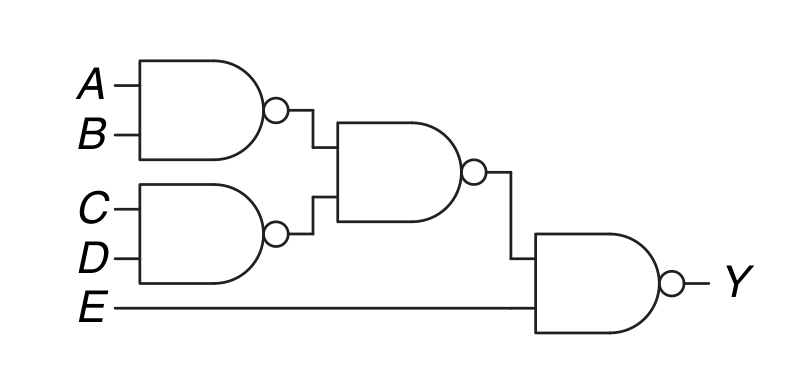
\includegraphics[width=0.4\linewidth]{./fig/fig2.83-circuit.png} 
\end{prob}
\newpage

\begin{prob}
  Describe how tri-state and open-collector outputs are different from totem-
  pole outputs using NMOS NOR gate as an example (10 marks).
\end{prob}
\newpage

\begin{prob}
  Assume that the inverter in the given circuit has a propagation delay of 5 ns and the
  AND gate has a propagation delay of 10 ns. Draw a timing diagram for the circuit
  showing X, Y, and Z. Assume that X is initially 0, Y is initially 1, after 10 ns X
  becomes 1 for 80 ns, and then X is 0 again. (20 marks)\\
  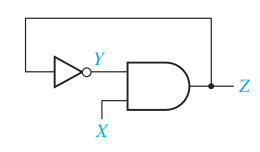
\includegraphics[width=0.4\linewidth]{./fig/fig-not-AND-latch.png}
\end{prob}
\newpage

\begin{prob}
  A latch can be constructed from an OR gate, an AND gate, and an inverter con-
  nected as follows: \\
  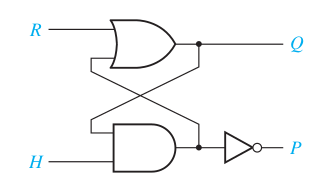
\includegraphics[width=0.4\linewidth]{./fig/or-AND-latch.png}\\
  \begin{enumerate}
    \item  What restriction must be placed on R and H so that P will always equal Q
    (under steady-state conditions) (10 marks)?
  \item Construct a characteristic (next-state) table and derive the
    corresponding characteristic equation for the latch (5 marks).
  \item Complete the following timing diagram for the latch (5 marks)\\
    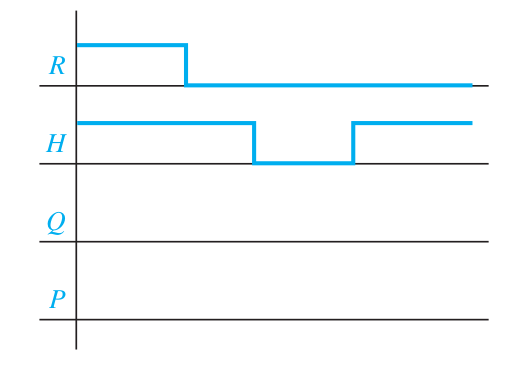
\includegraphics[width=0.4\linewidth]{./fig/timing-diagram.png}
  \end{enumerate}
\end{prob}
\newpage

\begin{prob}
  Design a 4-bit BCD counter that counts from 0000, to 1001 and then loops back
  to 0000 (20 marks).
  (Yet to be covered in class).\\
  \begin{enumerate}
  \item Draw its state transition diagram and table
  \item Design the circuit using a D flip-flop.
  \end{enumerate}
\end{prob}
\newpage

\begin{prob}
  Design a 3-bit modulo 8 Gray counter that counts from 000, to 111 and then loops back
  to 0000. (A modulo N counter counts from 0 to $N-1$) (20 marks).
  (Yet to be covered in class).\\
  \begin{enumerate}
  \item Draw its state transition diagram and table
  \item Design the circuit using a D flip-flop.
  \end{enumerate}
\end{prob}